\section{Introduction}\label{sec:intro}

Data agents convert natural-language questions into executable data
pipelines. They discover sources, inspect schemas, write SQL or Python
programs, repair execution errors, and report computed answers with
supporting evidence \citep{kramabench2025,dabstep2025,lakeqa2026}.
This workflow changes the object of verification. A reported value may
occur in no source file because it is produced by filtering, joining,
and aggregation. Auditing a computed answer therefore requires evidence
about the execution that produced it, rather than only evidence containing
related text or values.

\etitle{Running example.}
A KramaBench question asks for the mean number of identity-theft reports
among metropolitan areas whose 2023 population exceeds one million. The
agent declares 17 CSV files: one national identity-theft table and 16
state-level identity-theft tables. Its final Python program instead reads
the national table and 16 state-level fraud-and-other tables. It uses the
latter to construct a normalized metropolitan-area name set, infers
population as reports divided by the reporting rate per 100,000 times
$100{,}000$, retains 14 rows, and returns
$150{,}138/14=10{,}724.1429$, exactly the stated answer. However, 16 of
the 17 observed reads lie outside the declared evidence view. Restricted
replay over the declared files exits normally with
\texttt{\{"main-task": null\}}, leaving no output comparable with the
stated answer. A different failure remains possible after successful
replay: a program may use the wrong aggregation, predicate, or scope while
preserving the current output.

These failures induce three audit relations. \emph{Evidence
authorization} compares declared evidence with observed host reads.
\emph{Execution reproducibility} tests whether the final program
reproduces the stated answer within the authorized evidence view.
\emph{Semantic correctness} tests whether the program implements the
task specification. The first two relations admit deterministic trace and
execution witnesses; the third requires a task-specific specification,
such as reference SQL, executable constraints, database variants,
metamorphic relations, or human judgement. Figure~\ref{fig:teaser}
summarizes the three relations and their independent status outputs.

\begin{figure}[t]
\centering
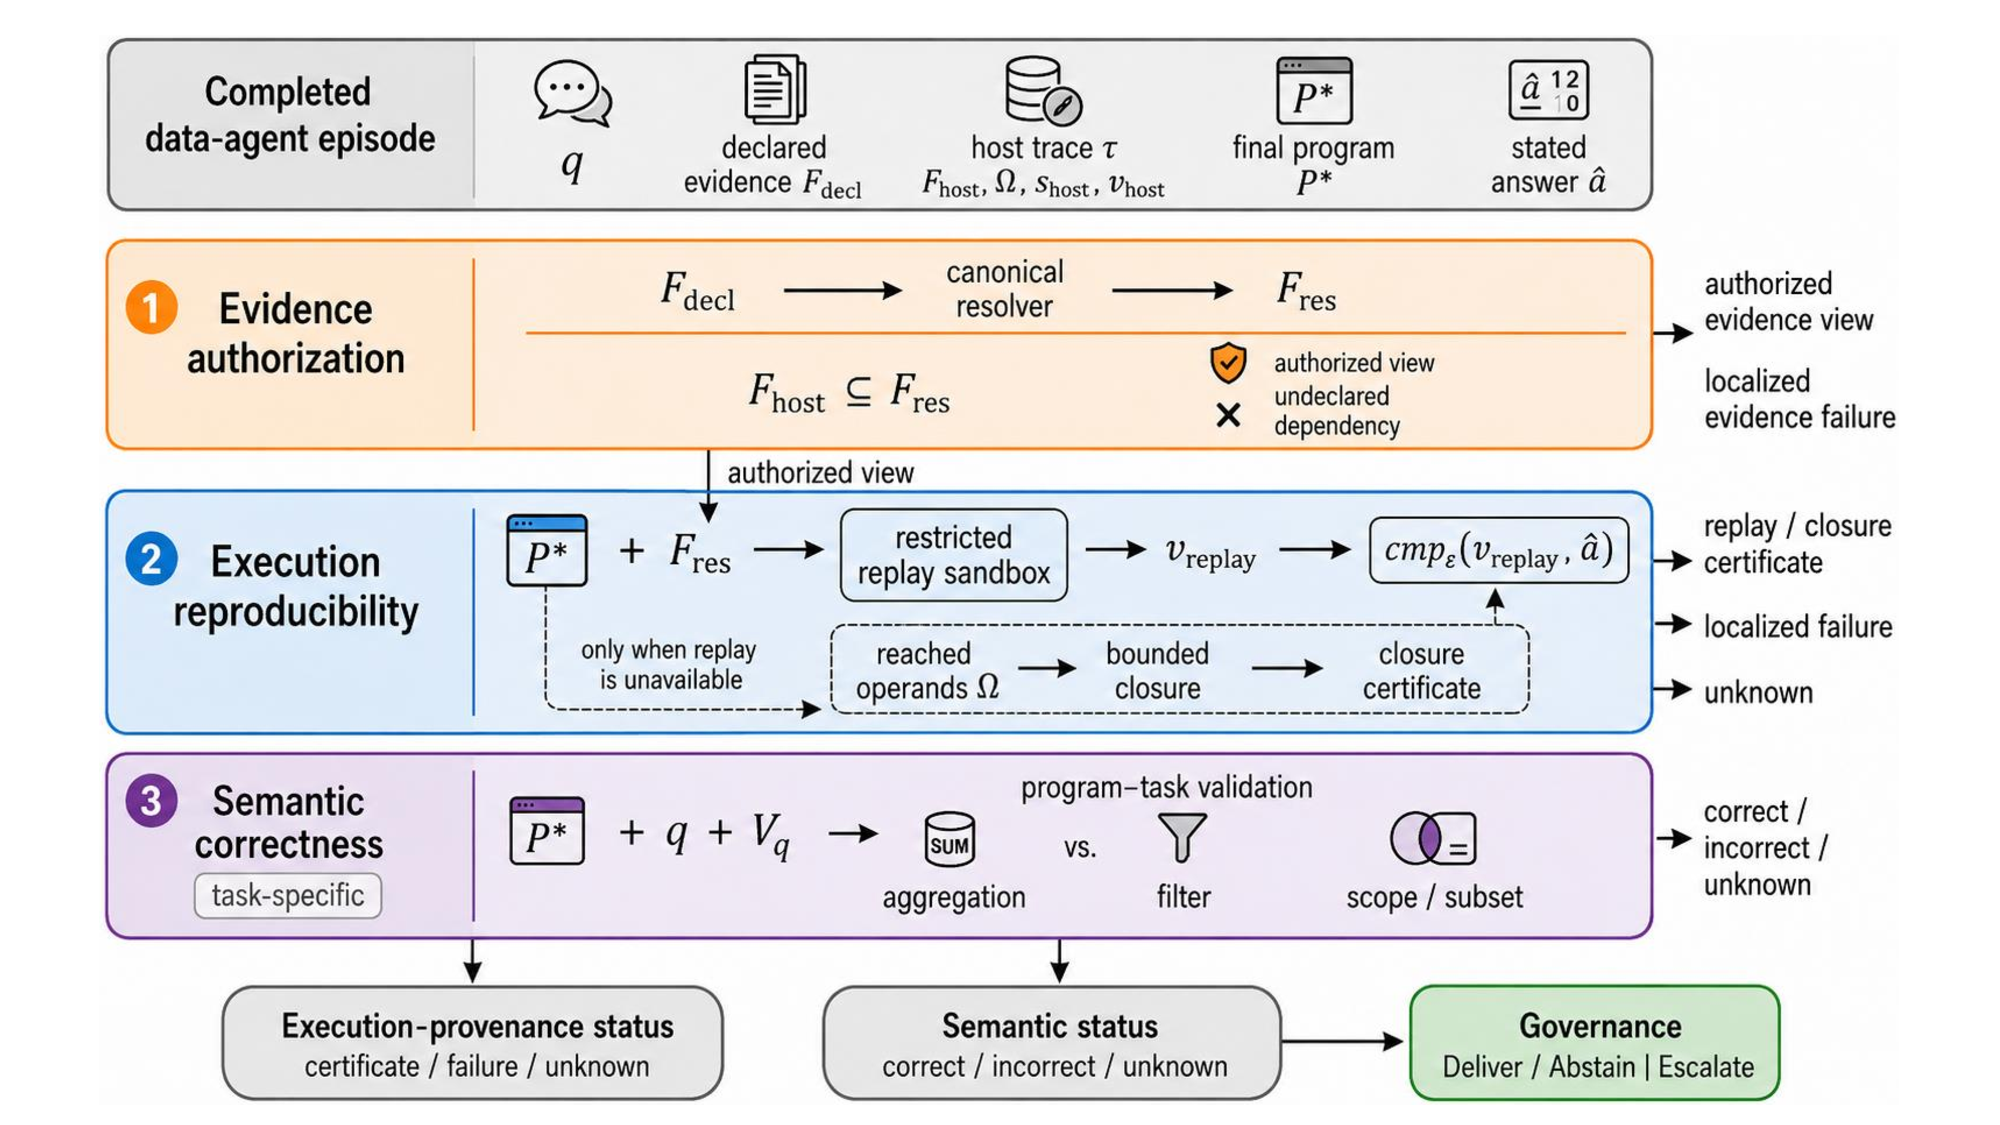
\includegraphics[width=\columnwidth]{teaser-v3.pdf}
\caption{%
Three relations required to audit a computed data-agent answer. Evidence
authorization establishes the permitted evidence view, and execution
reproducibility tests whether the final program reproduces the stated
answer within that view. Task-specific semantic validation independently
evaluates the question--program relation. Governance combines the
resulting provenance and semantic statuses.}
\label{fig:teaser}
\end{figure}

Existing methods address adjacent parts of this chain. Citation metrics
evaluate textual support \citep{gao2023alce,min2023factscore}. Database
provenance represents how a known query output depends on input tuples
\citep{green2007provenance,cheney2009provenance,
amsterdamer2011aggregate}, while script-provenance systems capture
runtime dependencies in controlled environments
\citep{murta2014noworkflow,namaki2020vamsa}. Agent benchmarks and
model-based judges evaluate final utility or interaction risk
\citep{ruan2024toolemu,debenedetti2024agentdojo,kramabench2025,
sana2026}. They do not provide a deterministic per-answer witness that
jointly connects the final program, stated answer, declared evidence, and
observed reads of a completed data-agent episode.

We introduce \ledger, a deterministic post-execution audit layer for
computed data-agent answers. \ledger freezes the final episode, resolves
declared evidence, reconciles host reads, and replays the final program
inside the resolved evidence view. It returns a replay certificate, a
localized failure, or unknown; when replay is unavailable, bounded closure
over program-reached operands provides a derivation witness. A separate
task-specific interface produces an independent semantic status. A
governance policy then combines the provenance and semantic statuses for
delivery, abstention, or escalation.

We make four contributions.
\begin{enumerate}
    \setlength{\itemsep}{0pt}
    \setlength{\parskip}{0pt}

    \item \textbf{Problem formulation.}
    We formulate post-execution auditing through evidence authorization,
    execution reproducibility, and semantic correctness, with an explicit
    trace contract, trusted computing base, failure semantics, and unknown
    outcome.

    \item \textbf{Theory.}
    We establish the relative soundness of citation-restricted replay,
    prove completeness of the bounded operand fallback within its operation
    and depth limits, and formalize why execution-provenance consistency
    does not imply semantic correctness.

    \item \textbf{Method.}
    We develop \ledger, combining canonical evidence resolution,
    read reconciliation, restricted replay, type-aware output comparison,
    operand-constrained closure, and an independent task-specific semantic
    interface. Each outcome carries a machine-readable witness or an
    explicit unknown status.

    \item \textbf{Evaluation.}
    We evaluate the three relations across controlled SQL perturbations,
    program-labelled numerical reasoning, and live data-agent episodes.
    \ledger detects same-output program changes, recovers
    89.6--93.3\% of reference derivations while rejecting
    96.1--97.2\% of cross-example unsupported answers, and improves the
    quality of replay-selected live answers at partial coverage.
\end{enumerate}
